\section{Códigos de Integración}

Para trabajar de una manera más eficiente se desarrollaron dos códigos separados
basado en su funcionalidad: unos scripts en Octave, la cual facilita operaciones
matemáticas y la creación de gráficas de una manera más declarativa, y un código
en C++, el cual ofrece mayor control sobre las instrucciones que debe correr el
programa y mayor extensibilidad. Los scripts de Octave fueron utilizados para
las soluciones analíticas para el modelo descrito en la sección
\ref{sec:modeloAnalitico}, mientras que el código de C++ fue utilizado para el
modelo C7 (sección \ref{sec:c7Modelo}). Ambas soluciones fueron graficadas
usando los scripts de Octave. El código completo se puede encontrar y descargar
del repositorio de GitHub
\href{https://github.com/KnightIV/EquilibrioHidrostatico}{EquilibrioHidrostatico}.

\subsection{Solución Analítica}

\subsubsection{Implementación del Código}
Las soluciones para el modelo analítico del equilibrio hidrostático en la
fotosfera del Sol están implementadas en el archivo
\verb|Graficas_EcuacionIdeal.m|. Aquí se definen las ecuaciones descritas la
sección \ref{sec:modeloAnalitico} dependientes de la altitud, representada por
el arreglo \verb|z| de \verb|6000| entradas, representando las altitudes en
metros para las cuales se van a resolver las ecuaciones. Este arreglo está
declarado en la parte superior del código junto al resto de las constantes
físicas necesarias para resolver el problema. 

Estas soluciones no pueden ser generadas todas al mismo tiempo debido a su
acoplamiento entre si, por lo que fue necesario resolverlas en un orden
específico. Para encontrar la densidad con respecto a la altitud se necesita
saber la presión; la presión requiere la integral del perfil de temperatura. Una
vez que cada una haya sido calculada se puede incluir en la subsecuente
ecuación. Debido que el propósito principal de Octave es facilitar la evaluación
de expresiones matemáticas estas operaciones son implementadas de manera
declarativa, cuya notación no es muy diferente que su representación matemática. 

\subsubsection{Resultados}
Una vez terminado el cálculo de cada ecuación el mismo script se encarga de
graficar los resultados. Esto se hace por conveniencia, ya que los datos siguen
en la memoria del programa corriendo. Para hacer esta parte más modular se
separó la función de graficar a un archivo separado dentro del proyecto, llamado
igual que la función \verb|plot_data_helper.m|. Aparte de separar la lógica del
código, esto también permite usar esta subrutina en el script que acompaña la
solución numérica. Los perfiles de presión, temperatura, y densidad obtenidos
mediante una integración analítica se pueden ver en la figura
\ref{modeloAnaliticoResultadosGraficas}, en las cuales se puede observar el
perfil suave que tienen cada una de las funciones. 

\begin{figure}[!ht]
	\centering
	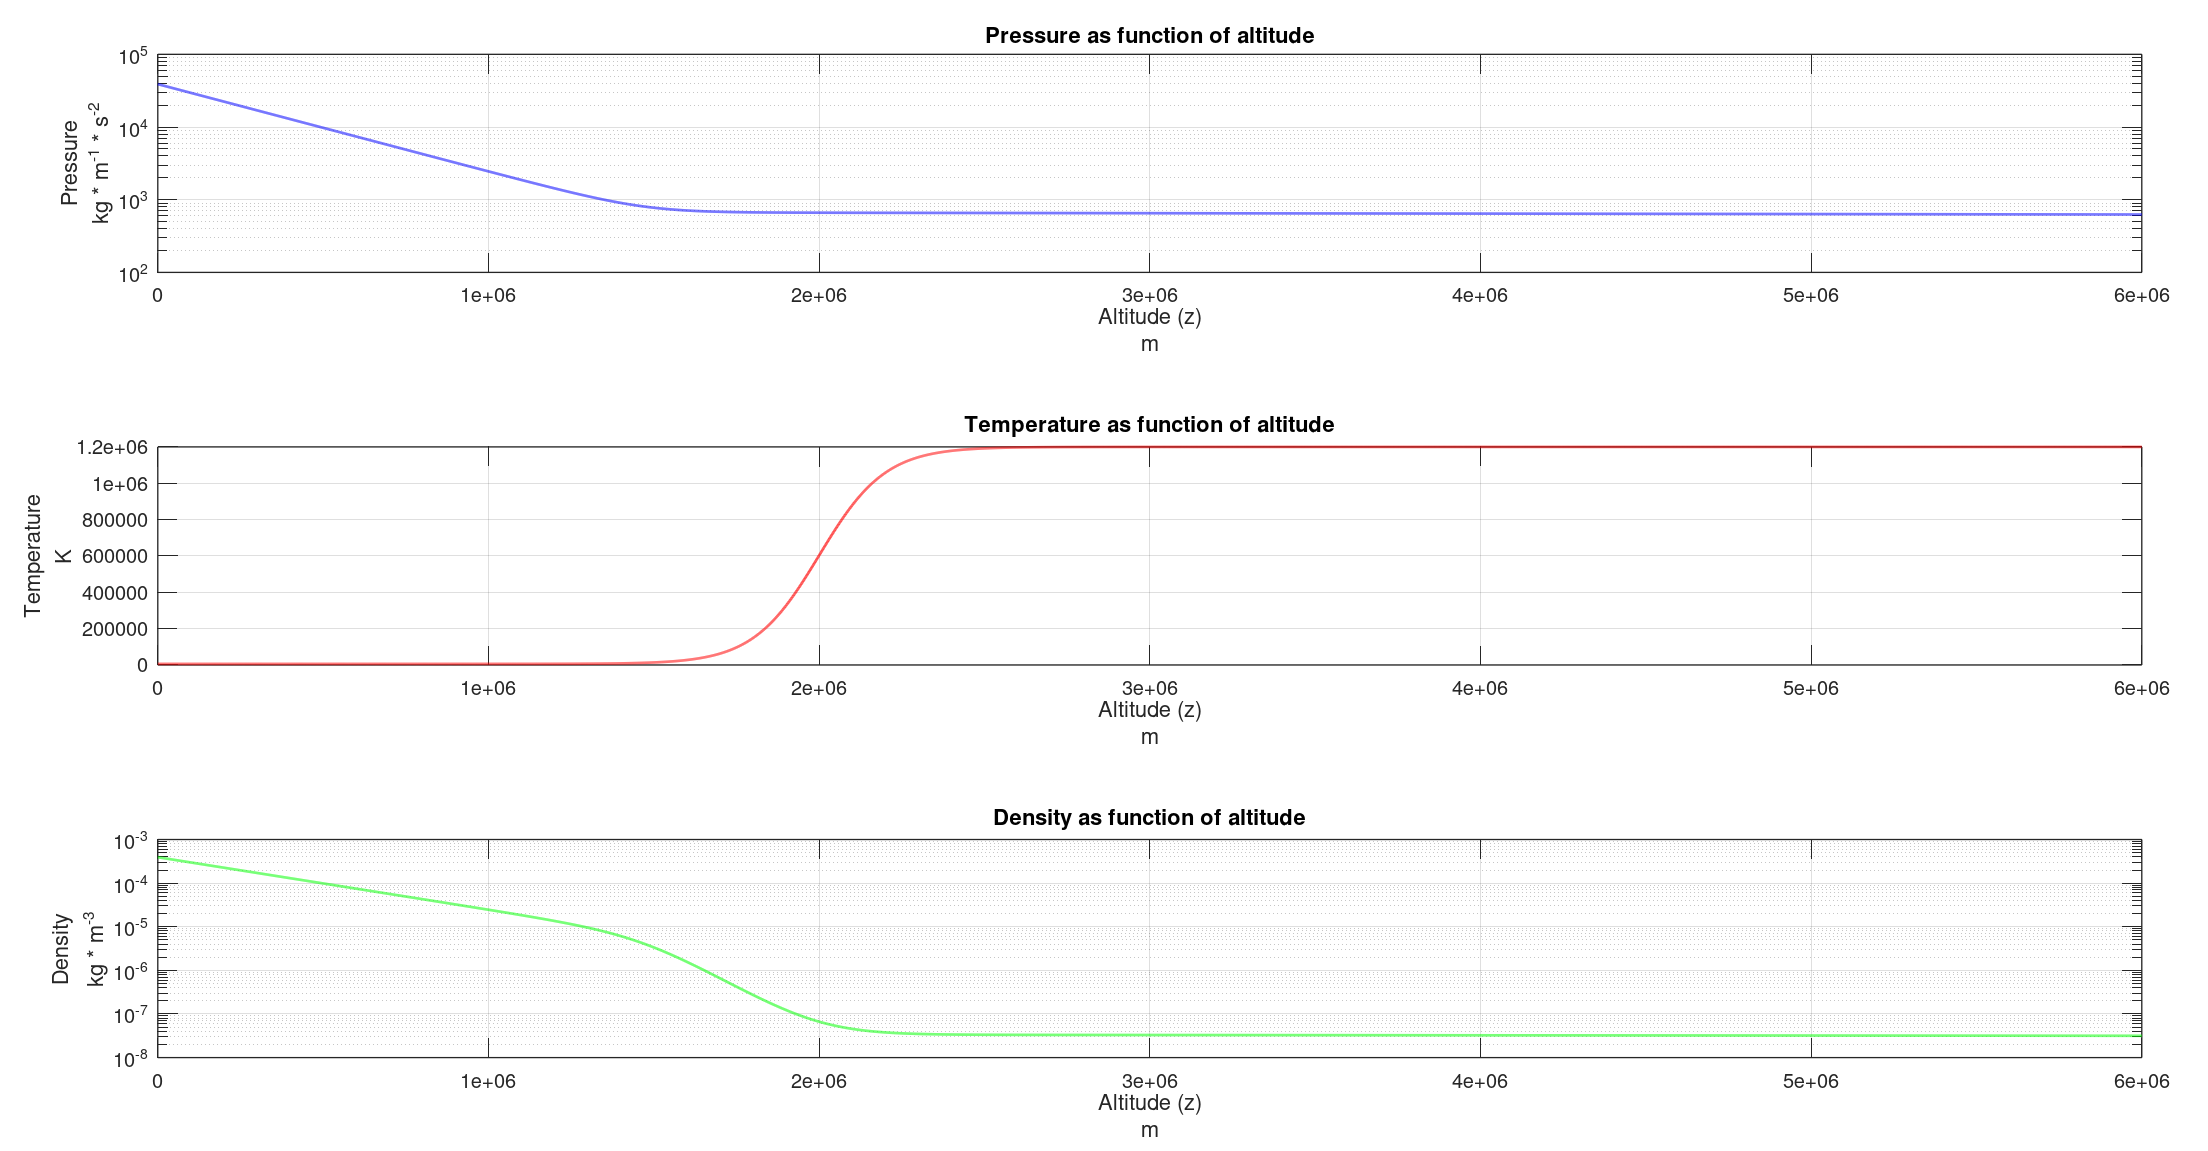
\includegraphics[scale=0.3]{Figuras/IntegracionAnaliticaGrafica.png}
	\caption{Perfiles de presión, temperatura, y densidad del plasma en la fotosfera y la región de transición a la corona.}
	\label{modeloAnaliticoResultadosGraficas}
\end{figure}

\subsection{Solución Numérica del Modelo C7}

\subsubsection{Implementación del Código}
A diferencia del código utilizado para la integración de las ecuaciones
analíticas, el modelo C7 fue resuelto con un código en C++. Este lenguaje fue
seleccionado por varias razones:

\begin{itemize}
	\item Habilidad de programar módulos por separado, incluyendo compilación.
	Esta fue la razón principal por la cual está escrita en C++, dejando abierta
	la posibilidad de implementar el código de integración numérica para que sea
	ejecutable en un procesador de gráficos (GPU). 
	\item Mayor control sobre las operaciones implementadas.
 	\item Compatibilidad entre Windows y Linux sin necesitar de varias
 	dependencias, con la excepción de herramientas de compilación.
\end{itemize}

El proyecto en si consiste de dos sub-proyectos, cada uno responsable de
diferentes funciones. El proyecto ejecutable, \verb|EquilibrioHidrostatico|,
contiene la rutina principal (la función \verb|main| requerida en todo
ejecutable escrito en C++) del programa, la cual hace llamadas a los módulos de
integración y extracción de datos descritos en las siguientes secciones. 

Una de las características principales de este código es que todos los datos los
mantiene en su memoria durante la ejecución del programa, en vez de calcular los
valores necesarios para cada altitud e escribir estos a un archivo
inmediatamente. //TODO: keep going

\subsubsection{\verb|EQHS_Data|}
Este módulo es el responsable de 